\item [3.1] Consider Fig \ref{fig: basis}.
What is the representation of the vector $\mathbf{x}$  with
respect to the basis $[\mathbf{q_1}, \mathbf{i_2}]$?
What is the representation of $\mathbf{q_1}$ with respect to
the basis $[\mathbf{i_2}, \mathbf{q_2}]$

\begin{figure}[htb!]
\centering
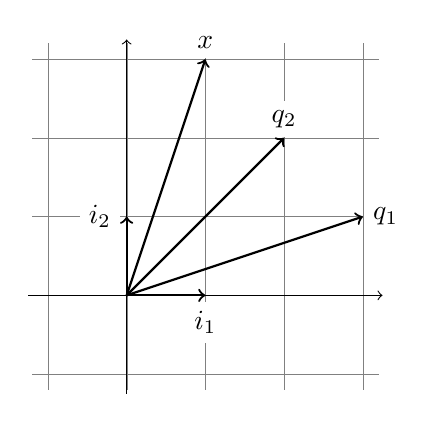
\begin{tikzpicture}[scale=1]
 \draw[step=1cm, gray, ultra thin] (-1.2,-1.2) grid (3.2,3.2);
  \draw[->, thin] (-1.25,0) -- (3.25,0) coordinate (x axis);
 \draw[->, thin] (0,-1.25) -- (0,3.25) coordinate (y axis);
%
 \draw[->, thick] (0,0) -- (1,0) node[below=2pt, fill=white]{$i_1$};
 \draw[->, thick] (0,0) -- (0,1) node[left=2pt, fill=white]{$i_2$};
%
\draw[->, thick] (0,0) -- (3,1) node[right, fill=white]{$q_1$};
\draw[->, thick] (0,0) -- (2,2) node[above, fill=white]{$q_2$};
%
\draw[->, thick] (0,0) -- (1,3) node[above, fill=white]{$x$};
   \end{tikzpicture}

 \caption{Different representations of vector x.}
 \label{fig: basis}
\end{figure}


Given the vector $\mathbf{x} = [1 \; 3]'$, we search for a
linear combination of $[ \mathbf{q_1} \; \mathbf{i_2} ]$
to represent $\mathbf{x}$ in that basis.

\begin{equation*}
 \mathbf{x} = \begin{bmatrix}
                1\\3
               \end{bmatrix}
            = [\mathbf{q_1} \; \mathbf{i_2} ] \begin{bmatrix}
                                                \alpha_1 \\ \alpha_2
                                               \end{bmatrix}
\end{equation*}

We solve this equation for $[\alpha_1 \; \alpha_2]'$.

\begin{align*}
\begin{bmatrix}
 1 \\3
\end{bmatrix}
& =
\begin{bmatrix}
 3 & 0\\
 1 & 1
\end{bmatrix}
\begin{bmatrix}
 \alpha_1 \\ \alpha_2
\end{bmatrix}\\
%
\begin{bmatrix}
 3 & 0\\
 1 & 1
\end{bmatrix}^{-1}
\begin{bmatrix}
 1 \\3
\end{bmatrix} &=
\begin{bmatrix}
 3 & 0\\
 1 & 1
\end{bmatrix}^{-1}
\begin{bmatrix}
 3 & 0\\
 1 & 1
\end{bmatrix}
\begin{bmatrix}
 \alpha_1 \\ \alpha_2
\end{bmatrix}\\
%
\begin{bmatrix}
 \alpha_1 \\ \alpha_2
\end{bmatrix}
 &=
 \begin{bmatrix}
1/3 \\
8/3
 \end{bmatrix}
\end{align*}

%%%%%%%%%%%%%%%%%%%%%%%%%%%%%%%%%%%%%%

Given the vector $\mathbf{q_1} = [3 \; 1]'$, we search for a
linear combination of $[ \mathbf{i_2} \; \mathbf{q_2} ]$
to represent $\mathbf{q_1}$ in that basis.

\begin{equation*}
 \mathbf{q_1} = \begin{bmatrix}
                3\\1
               \end{bmatrix}
            = [\mathbf{i_2} \; \mathbf{q_2} ] \begin{bmatrix}
                                                \beta_1 \\ \beta_2
                                               \end{bmatrix}
\end{equation*}

We solve this equation for $[\beta_1 \; \beta_2]'$.

\begin{align*}
\begin{bmatrix}
 3 \\1
\end{bmatrix}
& =
\begin{bmatrix}
 0 & 2\\
 1 & 2
\end{bmatrix}
\begin{bmatrix}
 \beta_1 \\ \beta_2
\end{bmatrix}\\
%
\begin{bmatrix}
 0 & 2\\
 1 & 2
\end{bmatrix}^{-1}
\begin{bmatrix}
 3 \\1
\end{bmatrix} &=
\begin{bmatrix}
 0 & 2\\
 1 & 2
\end{bmatrix}^{-1}
\begin{bmatrix}
 0 & 2\\
 1 & 2
\end{bmatrix}
\begin{bmatrix}
 \beta_1 \\ \beta_2
\end{bmatrix}\\
%
\begin{bmatrix}
 \beta_1 \\ \beta_2
\end{bmatrix}
 &=
 \begin{bmatrix}
-2 \\
3/2
 \end{bmatrix}
\end{align*}
